\documentclass{article}
\usepackage[utf8]{inputenc}

\title{NLP Report emoji prediction for text messages}
\author{Carsten Draschner, Maren Pielka, Jonas Weinz }
\date{July 2018}

\usepackage{natbib}
\usepackage{graphicx}
\usepackage{fontspec}
\usepackage{hyperref}

%\captionsetup[subfigure]{font=small,labelfont=scriptsize}
\usepackage{subcaption}
%\newfontfamily\DejaSans{DejaVu Sans}

\begin{document}

\maketitle

\tableofcontents

\section{Introduction}
For our lab project, we were investigating methods to predict suitable emojis for a text fragment taken from a chat conversation. At first we tested a naive approach without any Machine Learning, that compares the standard emoji descriptions to chat messages. This approach turned out to be effective for those emojis which are closely related to specific topics, but not for emotionally connected emojis. Then we tried out a more sophisticated method which uses feature extraction to train a classifier and optimized the parameters of the model. Finally, we merged both approaches together to get a model which is capable of predicting any kind of emojis.\\
Our idea and approach were inspired by the works of \citep{hallsmar2016}, \citep{novak2015} and \citep{zhao2017}, who were investigating a similar application, but with slightly different objectives and techniques.

\subsection{Motivation}
In a chat conversation, it is sometimes hard to predict the underlying emotion of the statement, if no emoticons are present. We want to tackle this problem by developing an emoji prediction system, which returns a suggestion for fitting emoticons, given a text fragment. It can be used as an auto-correct tool, to help your conversation partners understand your feelings better, or as an automated answering system, so that you will always have a suitable emoticon reaction to any message. \\
On the other hand, it might also be interesting to see which emotions are typically aligned with which emoticons, and vice versa.

\section{Naive Approach}
Initially we want to see how effective a very simple approach of Emoji prediction would be without any use of machine learning. Our first simple model uses some different processing layers. 
\begin{figure}[h!]
\centering
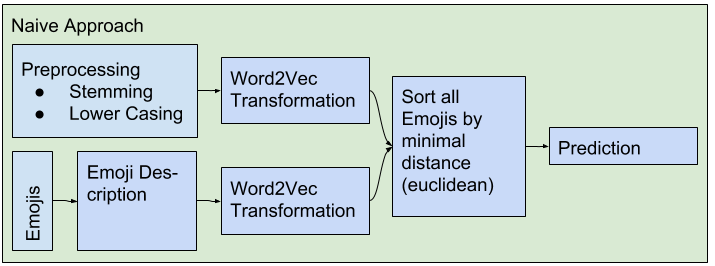
\includegraphics[scale=0.45]{images/naive_approach_1.png}
\caption{Naive Approach Outline}
\label{fig:naiveApproach}
\end{figure}
We want to predict for each of the messages in our dialog a set of best fitting emojis. So we want to match the text of the dialog messages to the emojis. 

\subsection{Matching of Messages to Emoji Specifications}
Emojis are non-textual information, so we have to assign a corresponding text representing these emojis. We are using the emoji specifications from \citep{EmojiSpec}.
\begin{figure}[h!]
\centering
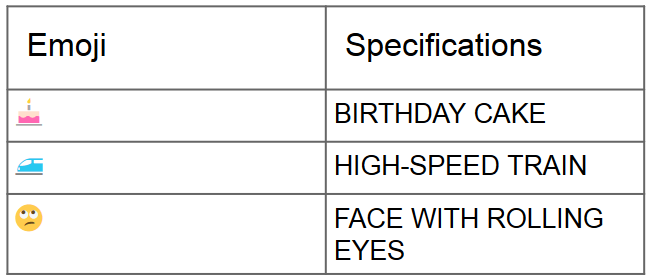
\includegraphics[scale=0.45]{images/emojiSpecs.png}
\caption{Examples for emoji specifications}
\label{fig:naiveApproach}
\end{figure}
We first preprocessed the messages and specifications using lowercasing and stopword removal. The text of the currently written message should then be matched to the emoji specification.

\subsubsection{Word2Vec/WordNet and Euclidean Distance}
\label{word2vec}
Word2Vec is a model which is trained on a text corpus to return a feature representation of words, based on their semantic similarity. So, if two words have a similar meaning, they are expected to be close to each other in feature space. It is also intended that the difference of two word vectors represents their relationship (for example, the difference between the vectors of “man” and “woman” should be similar to the difference between “king” and “queen”).\\
A similar concept is implemented by WordNet, a large lexical semantic web for the English language. It can be used to compute a synonym similarity between any pair of words, comparable to the Word2Vec similarity.\\
By using Word2Vec or WordNet representations we can compare the words in the messages with the emoji specification text. The Naive approach would be to compare each word representation of the message with each word of the emoji specifications pairwise. So for a message with n words and a specification of m words, you get n*m values between 0 and 1. Those values are further used to obtain one score for each message - specification pair (see section \ref{ranking}). \\
In the final implementation of our approach, we used WordNet similarities, because they yielded better results than Word2Vec.

\subsubsection{Ranking of Matching for Prediction}
\label{ranking}
In the future use of our prediction, we want to propose a small set of best fitting emojis matching to the currently written message. So we have to decide which are the best fitting messages. Considering the n*m vector as defined before, a “1” represents a perfect match and a “0” means that the strings don’t correlate.  We compare different approaches to rank these vectors:
\begin{itemize}
    \item sum of all values
    \item average of all values / mean
    \item $\frac{count(values>threshold)}{count(values)}$ for a given threshold with $0 < threshold < 1$
    \item $max(value)$
\end{itemize}
We compared these different ranking techniques and found that the threshold approach yields the best results, so we used it for our evaluation.

\subsection{Findings from the Naive Approach}
We discovered that it would be meaningful to distinguish between topic-related (e.g. soccer ball, card game) and emotion-related (“standard”) emojis. While the naive approach is relatively successful in predicting topic-related emojis, it fails in recognizing emotion-related emojis (like smileys). This is clear, since the emoji specification usually has no textual correlation with the respective message. So we concluded, to predict those emotions correctly, we would need a more advanced, Machine Learning based approach.

\section{Advanced Approach}
For the advanced approach, we tried different methods for matching text and emoticons.

\begin{figure}[h!]
\centering
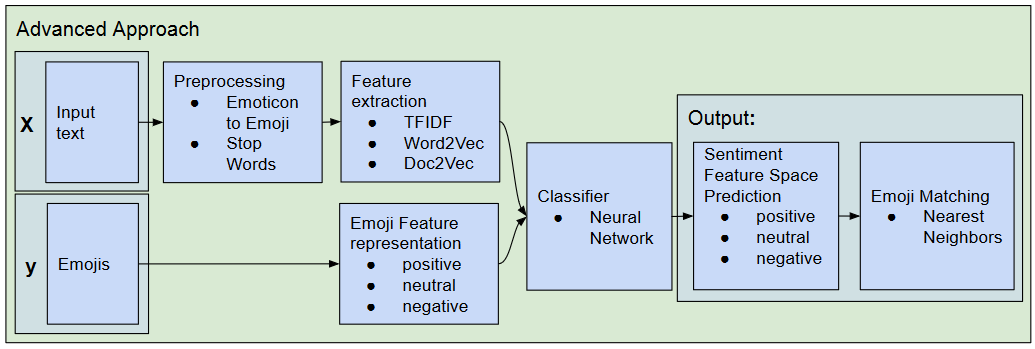
\includegraphics[scale=0.4]{images/advancedApproachOutline.png}
\caption{An overview of our conceptual design of the advanced approach}
\label{fig:merged_approach}
\end{figure}

\subsection{Preprocessing and Feature Extraction}
We used a publicly available dataset of 3 million Twitter messages from November and December 2017. In a first preprocessing step we got rid of unnecessary metadata and filtered out messages that are not either written in English or German. Also all messages without emojis were thrown away, and remaining messages were labeled by their emojis. For performance reasons we did this step with a combination of simple unix bash tools (e.g. sed and grep) and jq (\citep{jq}). \\
Then, inside Python, we preprocessed the input text and it's labels and tried two different approaches for a vector representation of the input text: TFIDF and Doc2Vec.

\subsubsection{TFIDF vectorization}
The TFIDF vectorizer derives a vector for an input sentence, based on the relative occurrences of the words in the sentence (term frequency), multiplied by a function that is decaying with their overall occurrence (inverse document frequency).
\[tfidf(d,t,D) = tf(t,d) * idf(t,D)\]
In this formula t is a term, d is the document (sentence) in which t occurs, and D is the collection of all documents.

\subsubsection{Doc2Vec vectorization}
Doc2Vec is a Feature Extraction model closely related to Word2Vec (see section \ref{word2vec}). It extends the model to not only represent single words, but complete documents (or, in case of our approach, twitter messages). For this purpose, an additional vector is introduced for each document and trained alongside with the word vectors. Only the document vectors are used for our model, as input to the classifier.

\subsection{Pipeline and Classifier}
We are using a sklearn Pipeline consisting of one vectorizer and a keras neural network as classifier. The vectorizer can either be a TFIDF- or doc2vec-vectorizer. We have built a jupyter notebook with an extendable interactive section to create a classifier and adjust the pipeline’s parameters.

\begin{figure}[h!]
\centering
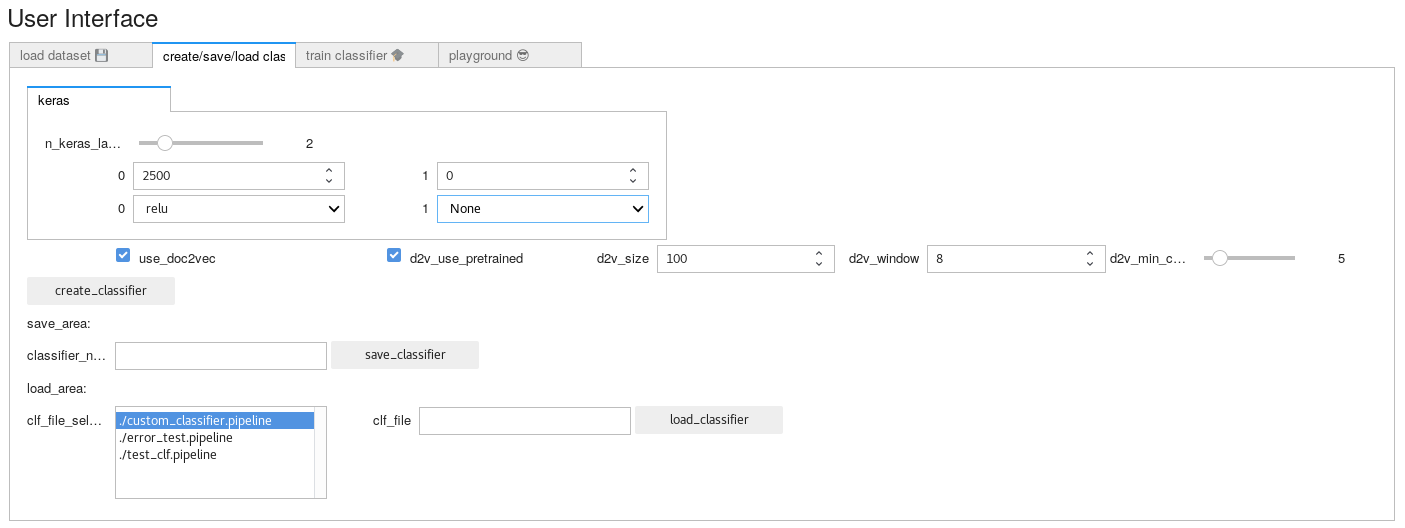
\includegraphics[width=\textwidth,height=\textheight,keepaspectratio]{images/Network-UI.png}
\caption{user interface for network creation}
\label{fig:NetworkUI}
\end{figure}

We can also load and save pipelines to disk.
Then data files can be selected to load twitter messages from our data pool. Since we have more messages in our data pool than we are able to hold in our RAM, we had to train multiple times. To achieve that we had to adjust the sklearn-pipeline such that it does not reset its steps when calling “fit” multiple times (especially for vectorizers like tfidf). Our solution was to override internal sklearn functions during runtime to avoid that.

\subsection{Emoji Representation}
In order to be able to compare emojis and evaluate the output of a classifier accurately, we need a representation in some feature space. We did this using an approach by \citep{novak2015}. The authors propose a mapping from emojis to a 3-dimensional, continuous vector space (see figure \ref{fig:emoji_space}). The dimensions are “Positive”, “Negative” and “Neutral”, which refer to the relative occurrences of the emoji in the respective context. Using this vector representation, we can calculate the Euclidean distance between any pair of emoticons. This distance can be used to implement a continuous error function, when dealing with the output of a classifier. It is likely to be more precise than a standard accuracy function, which would be 0 for any pair of emojis that do not match exactly.

\begin{figure}[h]
\centering
\begin{subfigure}{0.49\textwidth}
\centering
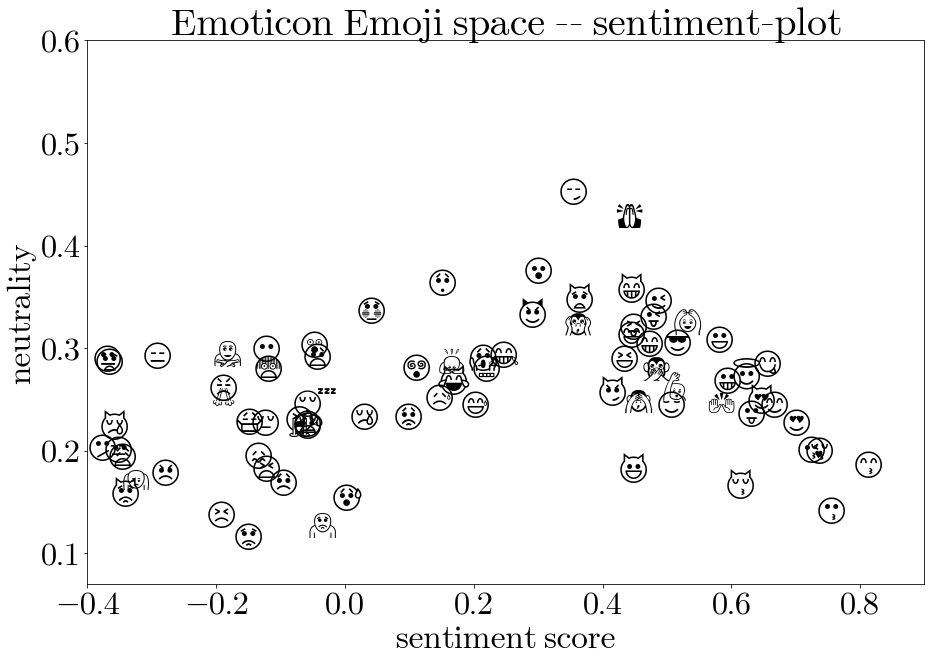
\includegraphics[width=0.9\linewidth]{images/Emoji-sn-plot.png}
\subcaption{sentiment-score / neutrality}
\end{subfigure}
\begin{subfigure}{0.49\textwidth}
\centering
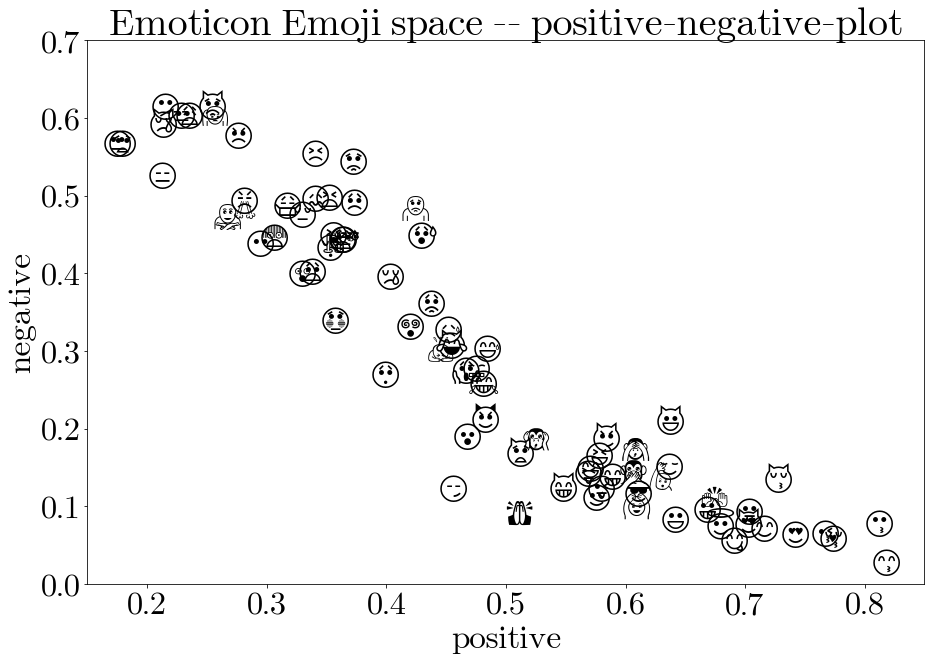
\includegraphics[width=0.9\linewidth]{images/Emoji-pn-plot.png}
\subcaption{positive / negative plot}
\end{subfigure}
\caption{Emoji Distribution in Sentiment Space. The sentiment score is defined by the difference of the positive and negative part}
\label{fig:emoji_space}
\end{figure}

\subsection{Problem Specification and Error Function}
Given the continuous representation of the emojis, the classification becomes a regression task. Regarding the error function, we measure the distance of the predicted point in feature space to the vector representation of 
the correct emoji.
\begin{figure}[h!]
\centering
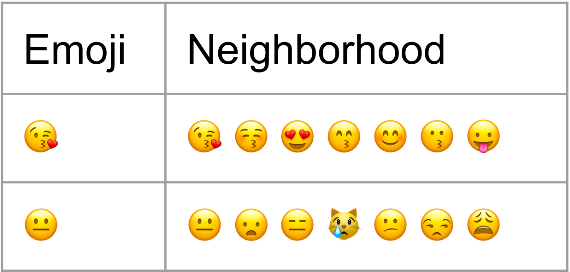
\includegraphics[scale=0.5]{images/closestEmojis}
\caption{Examples for some emojis and their nearest neighbors in the three dimensional feature space}
\end{figure}


\section{Merged Approach}
We decided to merge our Naive and our Advanced Approach to combine the advantages of both. For Sentiment Analysis we use our advanced approach, but for the topic related analysis we use our naive approach. 

\begin{figure}[h!]
\centering
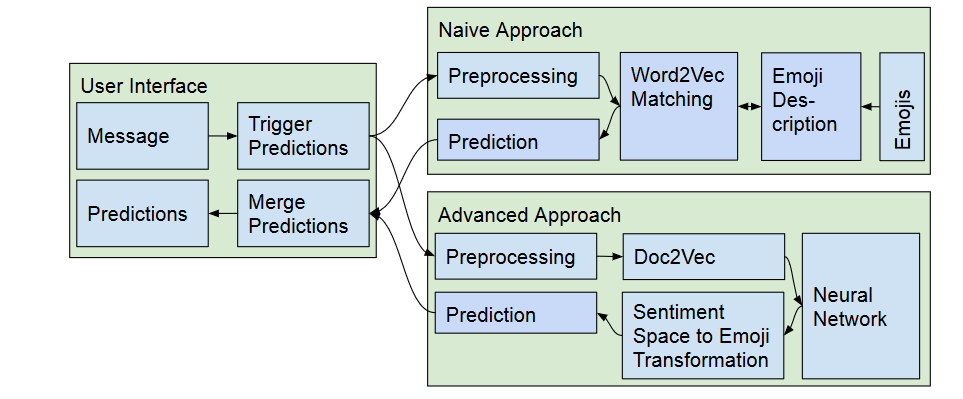
\includegraphics[scale=0.45]{images/mergedApproachOutline.png}
\caption{An overview of our conceptual design of the merged approach}
\label{fig:merged_approach}
\end{figure}

\subsection{User Interface}
To get in touch with the current state of our project, we designed a simple User Interface. It is inspired from the common appearance of chat or dialog systems on mobile devices. We decided to implement our own sketch UI because we want to have buttons for our predictions.

\subsubsection{Components}
Our User Interface provides the history of inserted messages in the top. As to the input from the user, we have a text field for messages which are online analysed for the best fitting predictions. Those are presented on the top of the text input field as buttons labeled with the predicted emojis.

\begin{figure}[h!]
\centering
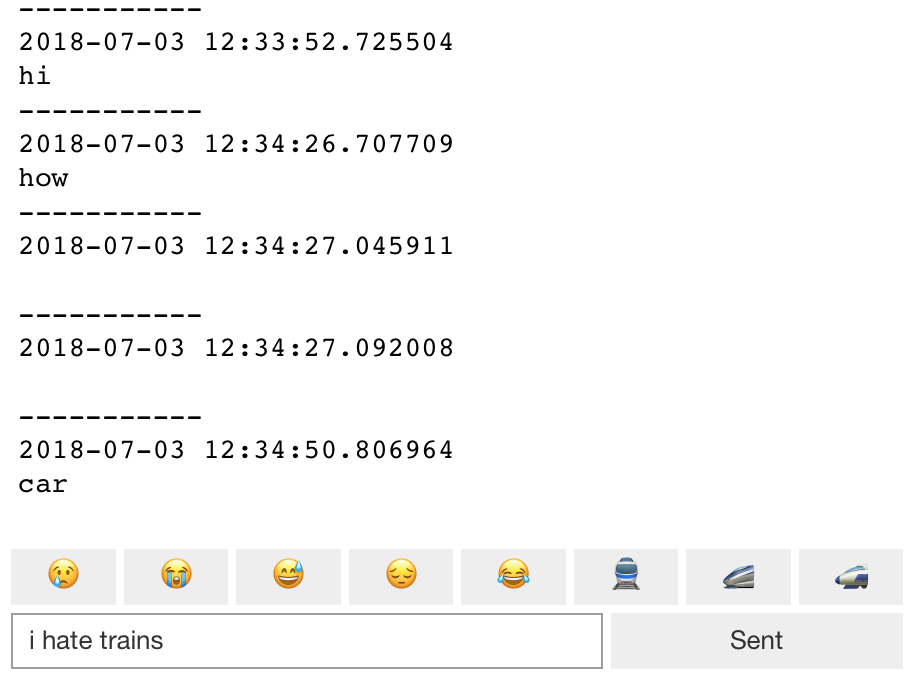
\includegraphics[scale=0.4]{images/user_interface}
\caption{Current Message: I hate trains; Result: 3 topic related predictions (maximum 4 allowed) showing emojis containing trains and 5 additional sentiment analysis predictions of emojis containing almost sad faces
}
\label{fig:user_interface}
\end{figure}

\subsubsection{Merge Predictions}
The interactive prediction results from the parallelly started prediction of both approaches. We’ve chosen to provide 8 predictions of best fitting emojis and a 50/50 split of these 8 possible predictions (4 sentiment, 4 topic). If there are too few topic related predictions, we fill up these positions by more sentiment related emojis. Also the set of emojis for prediction can be defined and is set to the top 20 most used emojis from our training set.

\subsubsection{Results from Use of User Interface}
We see that a merge of both approaches makes sense and offers a wider range with easier access to emojis compared to our usual use. But also as expected our sentiment analysis does not always provide the optimal expected emojis. In contrast to that, the naive approach provides meaningful emojis most of the time.

\section{Results}

\subsection{Comparison Approaches}
As mentioned before, the naive approach which was almost easy to implement, provided a good feedback for topic related emoji prediction. An improvement in speed was possible by switching from WordNet to Word2Vec implementation. For a sentiment analysis, this approach does not have enough capabilities because sentiments aren't hard coded in chat messages and thus won't be matched to emoji specifications. We designed the advanced approach to deal with this problem. The results were quite good for easy and kind of obvious messages but shows that we also got many false prediction when sentences are getting longer.

\subsection{Results of the Neural Network classifier}

For the final training we used a Neural Network with 3 hidden layers (5000, 2500 and 1000 neurons). As vectorizer we tested TFIDF and doc2vec. In comparison to TFIDF we had to train the doc2vec vectorizer on much more twitter samples until we get good results, but still then a pipeline using TFIDF performs better (see figure \ref{fig:error_plot}).

\begin{figure}[h!]

\begin{subfigure}[c]{\textwidth}
\begin{subfigure}[c]{0.5\textwidth}

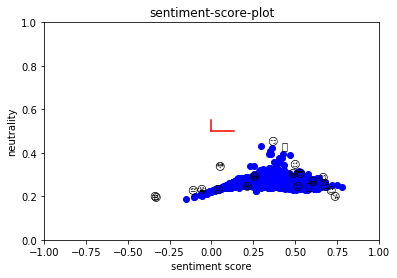
\includegraphics[width=0.9\textwidth]{images/tfidf_plot_01.png}


\end{subfigure}
\begin{subfigure}[c]{0.5\textwidth}

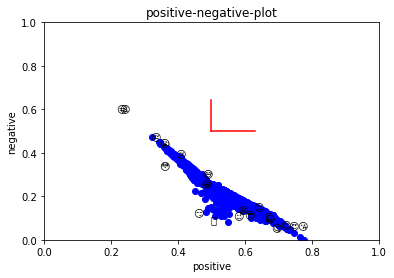
\includegraphics[width=0.9\textwidth]{images/tfidf_plot_02.png}
\end{subfigure}
\subcapture{prediction distribution with red mean-error bars}
\end{subfigure}
\begin{subfigure}[c]{\textwidth}
\centering
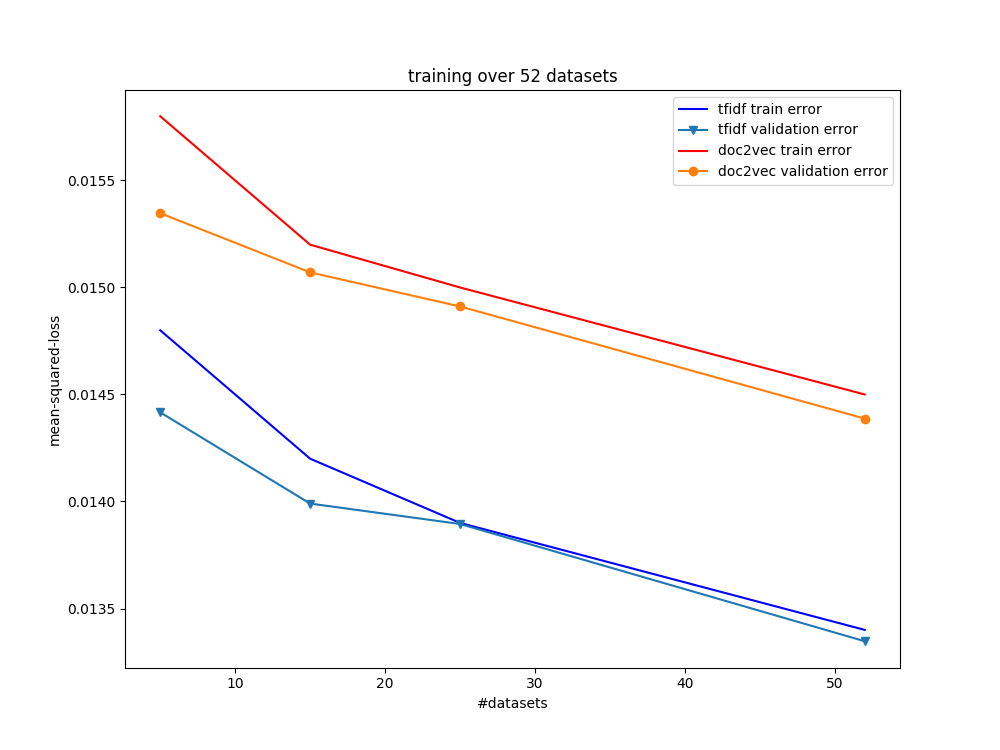
\includegraphics[width=0.5\textwidth]{images/train_valid_error.png}

\subcapture{Train and validadtion Error on the same network with TFIDF and doc2vec vectorizers. Shown here is the training of 2 months of archieved twitter data distributed over 54 data files. 52 were used for training, 2 for validation}
\end{subfigure}
\caption{Training Error Evaluation}
\label{fig:error_plot}
\end{figure}





\subsection{Evaluation}
It is not easy for us to present numeric values. This is due to the fact that we learn our sentiment as a regression problem. So we can provide loss over time. In context of sentiments this is not so intuitive. When using the user interface with an example input text and watching for the presented emojis we see intuitively a quite good matching. But we have to investigate for a good measurement of such problems.

\section{Discussion}
After finishing our project we have many ideas for further research where we could improve our approaches. On the one hand we have ideas for further tools or integration of additional software for a more efficient use of our data, on the other hand we see some limitations and problems based on design.

\subsection{Outlook}
In our group we discussed many more ideas, how we can improve our approaches. 
With  more time it could be interesting to offer the opportunity of using different languages as input. Also it could be interesting to use the 

\subsubsection{Chatbot}
A possible implementation of our approach would be a chatbot, which answers an input message with an emoji (and possibly an additional reply message). We implemented this function with a chat interface. The bot will always reply to the input message with the top-ranked emoji from our Advanced Approach.

\subsubsection{Multi Language}
For an integration in Messenger services or chat bots it would be interesting to offer the opportunity of language independence.

\subsubsection{Reinforcement Learning}
We could use the user input after predicting the most probable emojis. When a user selects a specific emojis with a less higher rank we could use this as a feedback for improving further predictions like in reinforcement learning or generating a new training sample.

\subsubsection{Irony}
In data from twitter or other social media, irony, sarcasm and other obfuscated sentiments are present. To analyze them and interprete the used emojis we have to build a deeper knowledge about the messages. To detect irony, we have to understand the messages content. Also we need to match this content to the writers knowledge. If we also could detect that a mismatch of the content in the written message and the authors knowledge base and in addition we expect that the author thinks we are able to understand that his message is intentionally wrong exposed, we could assume that it is maybe an ironic, sarcastic or trolling message.

\subsection{Limitations}
Also while implementing our approaches we see many limitations in our design and data. But we have to deal with it based on our time schedule. If we would have much more time we would investigate many of them. We want to give a short overview  to show where we think we lost some accuracy.

\subsubsection{Alternative evaluation with independent data}
\label{sec:alternative_eval}
One of the biggest issues with the Advanced Approach is that the mean squared error of the Neural Network is not so well interpretable. We tried to get a more intuitive performance estimate with an independent evaluation. We wrote 120 sentences by hand (60 topic- and 60 emotion-related). The emotion related sentences were labeled as to their basic emotion (positive or negative). Then we ran the Merged Approach on that data and evaluated the results of the Naive and the Advanced Approach separately.
\begin{figure}[h!]
\centering
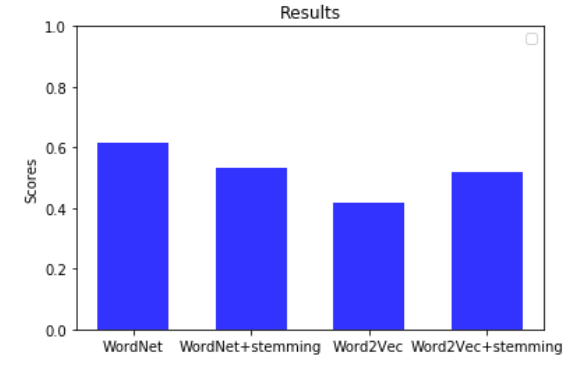
\includegraphics[scale=0.45]{images/naiveApproachEval.png}
\caption{Results of the Naive Approach on our own data, evaluated by hand}
\label{fig:naiveApproachEval}
\end{figure}
For the evaluation of the Naive Approach, we just counted the number of examples for which the algorithm returns at least one meaningful topic-emoji (normalized by the number of all examples). We also did a comparison between WordNet and Word2Vec with and without stemming, respectively. The results can be seen in figure \ref{fig:naiveApproachEval}. We inferred from this experiment that WordNet without stemming performs best for our data.\\
To evaluate the Advanced Approach, we compared the top 4 predicted emojis to our previously defined emotion labeling. If at least 2 of them correlated with the "true" sentiment, the example was considered a hit, otherwise a miss. Again, we counted the number of hits and divided it by the total number of examples. We did this for two classifiers, one of which used the TFIDF feature representation, and one the Doc2Vec representation. The classifier with TFIDF vectors got an accuracy score of 0.85, and the one with Doc2Vec 0.6. We excluded the by far most used emoji "Face with Tears of Joy" from this evaluation, because it was predicted by the classifier for almost every sentence and therefore not meaningful.\\
It is important to note that these scores are just rough estimations, which we obtained to get a better feeling for how well our approach performs. We did not include them in the official evaluation, as they are not an exact performance measure.

\subsubsection{Data}
Our twitter data is not a gold standard for text with a good sentiment labeling. Our prototype works with the used emojis to approximate the underlying sentiment. We think a larger set of Whats App data would be much more interesting because of a longer history of interaction with more honest writing of sentiments and thus less noise. So a more precise prediction could be possible based on more information about context. Also there seems to be too much noise in the emoji usage. So you can also see in figure \ref{fig:bad_cluster} that the predictions of our classifier performs not so good on general twitter messages. But the same classifier can work if there is clearly a strong sentiment in the message. As you can see in figure \ref{fig:good_cluster} is is possible to separate predictions of messages with positive and negative sentiments

\begin{figure}[h]
\centering
\begin{subfigure}{0.49\textwidth}
\centering
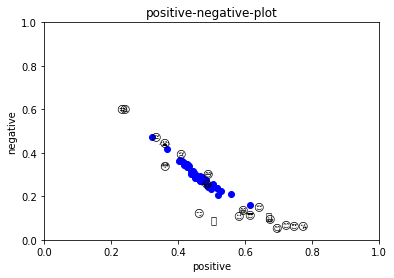
\includegraphics[width=0.9\linewidth]{images/pn-plot-sad.png}
\subcaption{positive / negative plot of sad Emoji}
\end{subfigure}
\begin{subfigure}{0.49\textwidth}
\centering
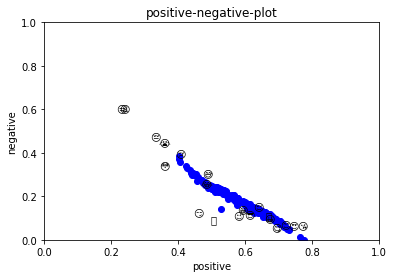
\includegraphics[width=0.9\linewidth]{images/pn-plot_kiss.png}
\subcaption{positive / negative plot of kissing Emoji}
\end{subfigure}
\caption{Example for bad predictions of our advanced classifier (TFIDF as vectorizer). Here we see predictions of our twitter-data validation set, left only with data which has a sad emoji as true label, right only data with the kissing emoji as true label. The two clusters are not separated in the Sentiment space}
\label{fig:bad_cluster}
\end{figure}

\begin{figure}[h]
\centering
\begin{subfigure}{0.49\textwidth}
\centering
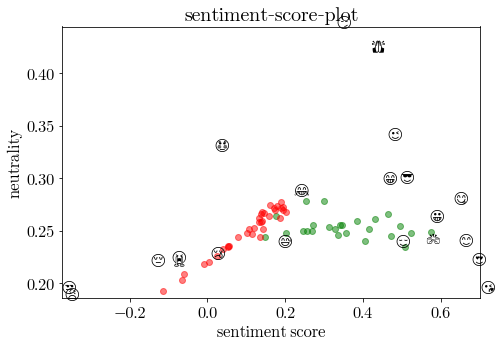
\includegraphics[width=0.9\linewidth]{images/sentiment-sn-plot.png}
\end{subfigure}
\begin{subfigure}{0.49\textwidth}
\centering
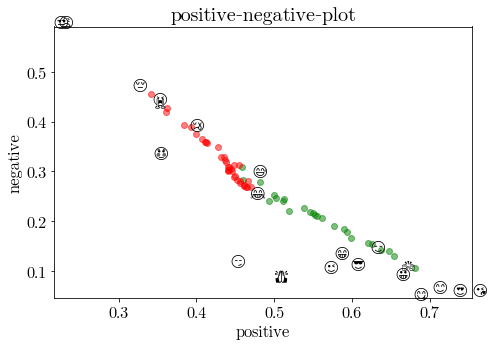
\includegraphics[width=0.9\linewidth]{images/sentiment-pn-plot.png}
\end{subfigure}
\caption{The same classifier as in figure \ref{fig:bad_cluster}, but here we see predictions of the sentiment data mentioned in section \ref{sec:alternative_eval}. Green are messages with a strong positive, Red with strong negative sentiment}
\label{fig:good_cluster}
\end{figure}

\subsubsection{Sentiment Space}
In or research of labeled twitter data and assignments of sentiments with emojis, we found a paper  which mapped  emojis occurring in a text to positive, negative or neutral classes (see \citep{novak2015}). Based on this data we built a 3-dimensional sentiment space. We evaluated this space with clustering and investigated for each emoji the nearest neighbours. This model offers us an alternative representation for multi-class classification (see section \ref{clustering}) in our Neural network, but isn't investigated much further. We also thought about alternative sentiment spaces but do not have enough time to investigate them. 

\paragraph{Emoji Clustering}
\label{clustering}
To analyze the data, we performed k-means clustering on the emoji representations in the three-dimensional feature space. We found that k = 5 yields meaningful clusters, which represent clearly distinguishable types of emojis.
\begin{figure}[h!]
\centering
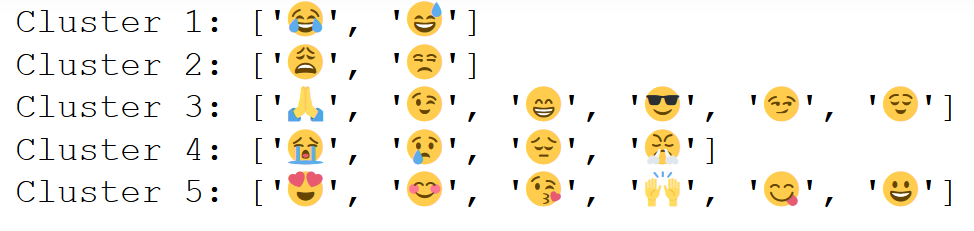
\includegraphics[scale=0.45]{images/clusters}
\caption{Cluster representation of the 20 most used emojis}
\label{fig:clusters}
\end{figure}
A rough classification of the clusters - as to their represented emotions - would be:
\begin{itemize}
    \item Cluster 1: Joy / Fun 
    \item Cluster 2: Anger / Desperation
    \item Cluster 3: Miscellaneous
    \item Cluster 4: Sadness / Rage
    \item Cluster 5: Love / Happiness
\end{itemize}
This representation can be helpful, when interpreting classification results. If we want to know how good a result is, we can check if its closest representation is in the same cluster as the correct emoji. One should keep in mind though, that this is not an exact performance measure. Therefore we did not include it in our evaluation.

\subsubsection{Trolls and Irony}
Possible misusage and misinterpretation of used twitter data based on not detecting trolls or ironic statements could lead to a wrong sentiment assignment. This problem could be a large one in context social media like Twitter or reddit where a large community of users are trolls.

\bibliographystyle{plain}
\bibliography{references}


\end{document}